\documentclass[a4paper,12pt]{article}
\usepackage{amsmath,amssymb,mathtools}
\usepackage{parskip}
\usepackage[utf8]{inputenc}
\usepackage[T1]{fontenc}
\usepackage{charter}
\usepackage{graphicx}
\usepackage[left=2.0cm,right=2.0cm,top=2.0cm,bottom=2.0cm]{geometry}
\usepackage[labelfont=bf]{caption}
\usepackage{subcaption}
\usepackage{setspace}
\setlength{\parskip}{10pt}

\title{Remaining Work}
\author{Shaon Samanta}
\date{}

%\DeclareCaptionLabelFormat{caps}{\textbf{FIG~#2:}}
%\captionsetup[figure]{labelformat=caps,labelsep=space}

\begin{document}
\onehalfspacing
\makeatletter
\def\@maketitle{
\begin{center}
\vspace*{0.4cm}
{\Huge \@title }\\[0.5ex]
{\large \bfseries \textit{Modulation instability in semiconductor quantum dots (Y-type excitation scheme)} }\\[1.3ex]
{\@author }\\[5ex]
\end{center}}
\makeatother

%\maketitle

\section{Linear and Non-linear Susceptibilities}

\noindent
\begin{figure}[h]
  \centering
  \begin{minipage}[t]{0.48\textwidth}
    \centering
    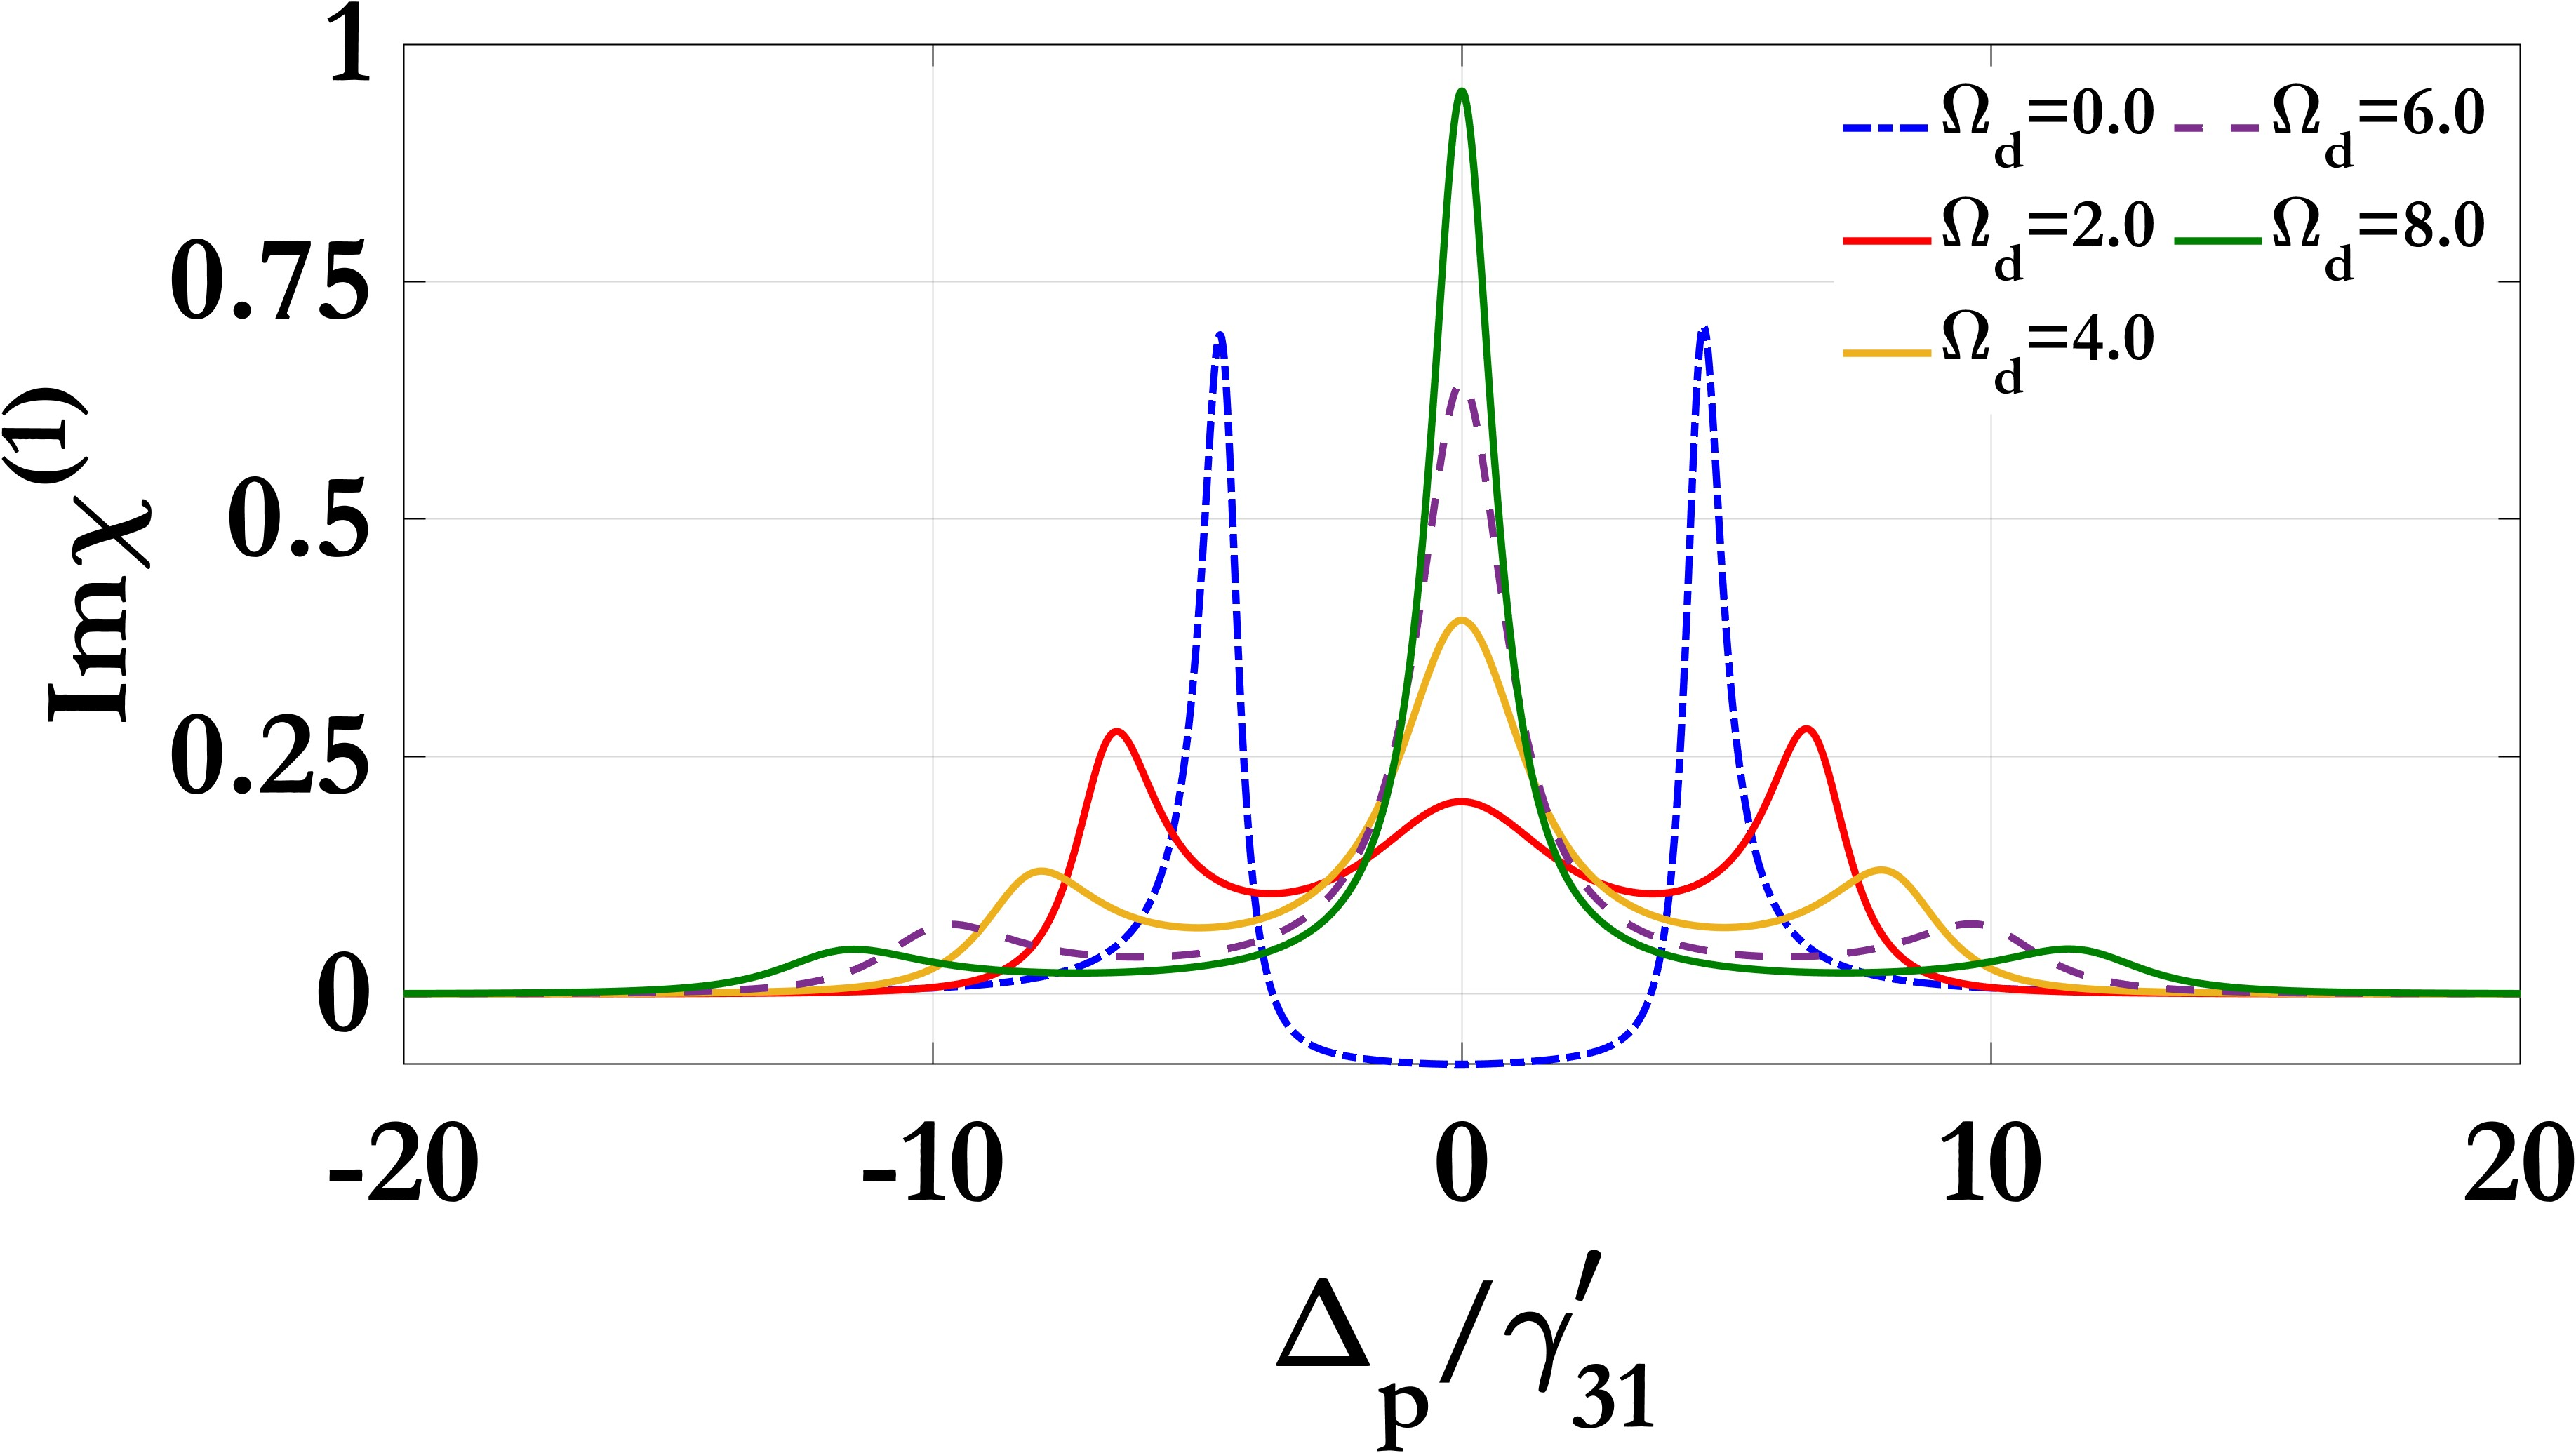
\includegraphics[width=\linewidth]{Plots/Img_chi1_Omega_d.jpeg}
    \subcaption{}
  \end{minipage}%
  \hfill
  \begin{minipage}[t]{0.48\textwidth}
    \centering
    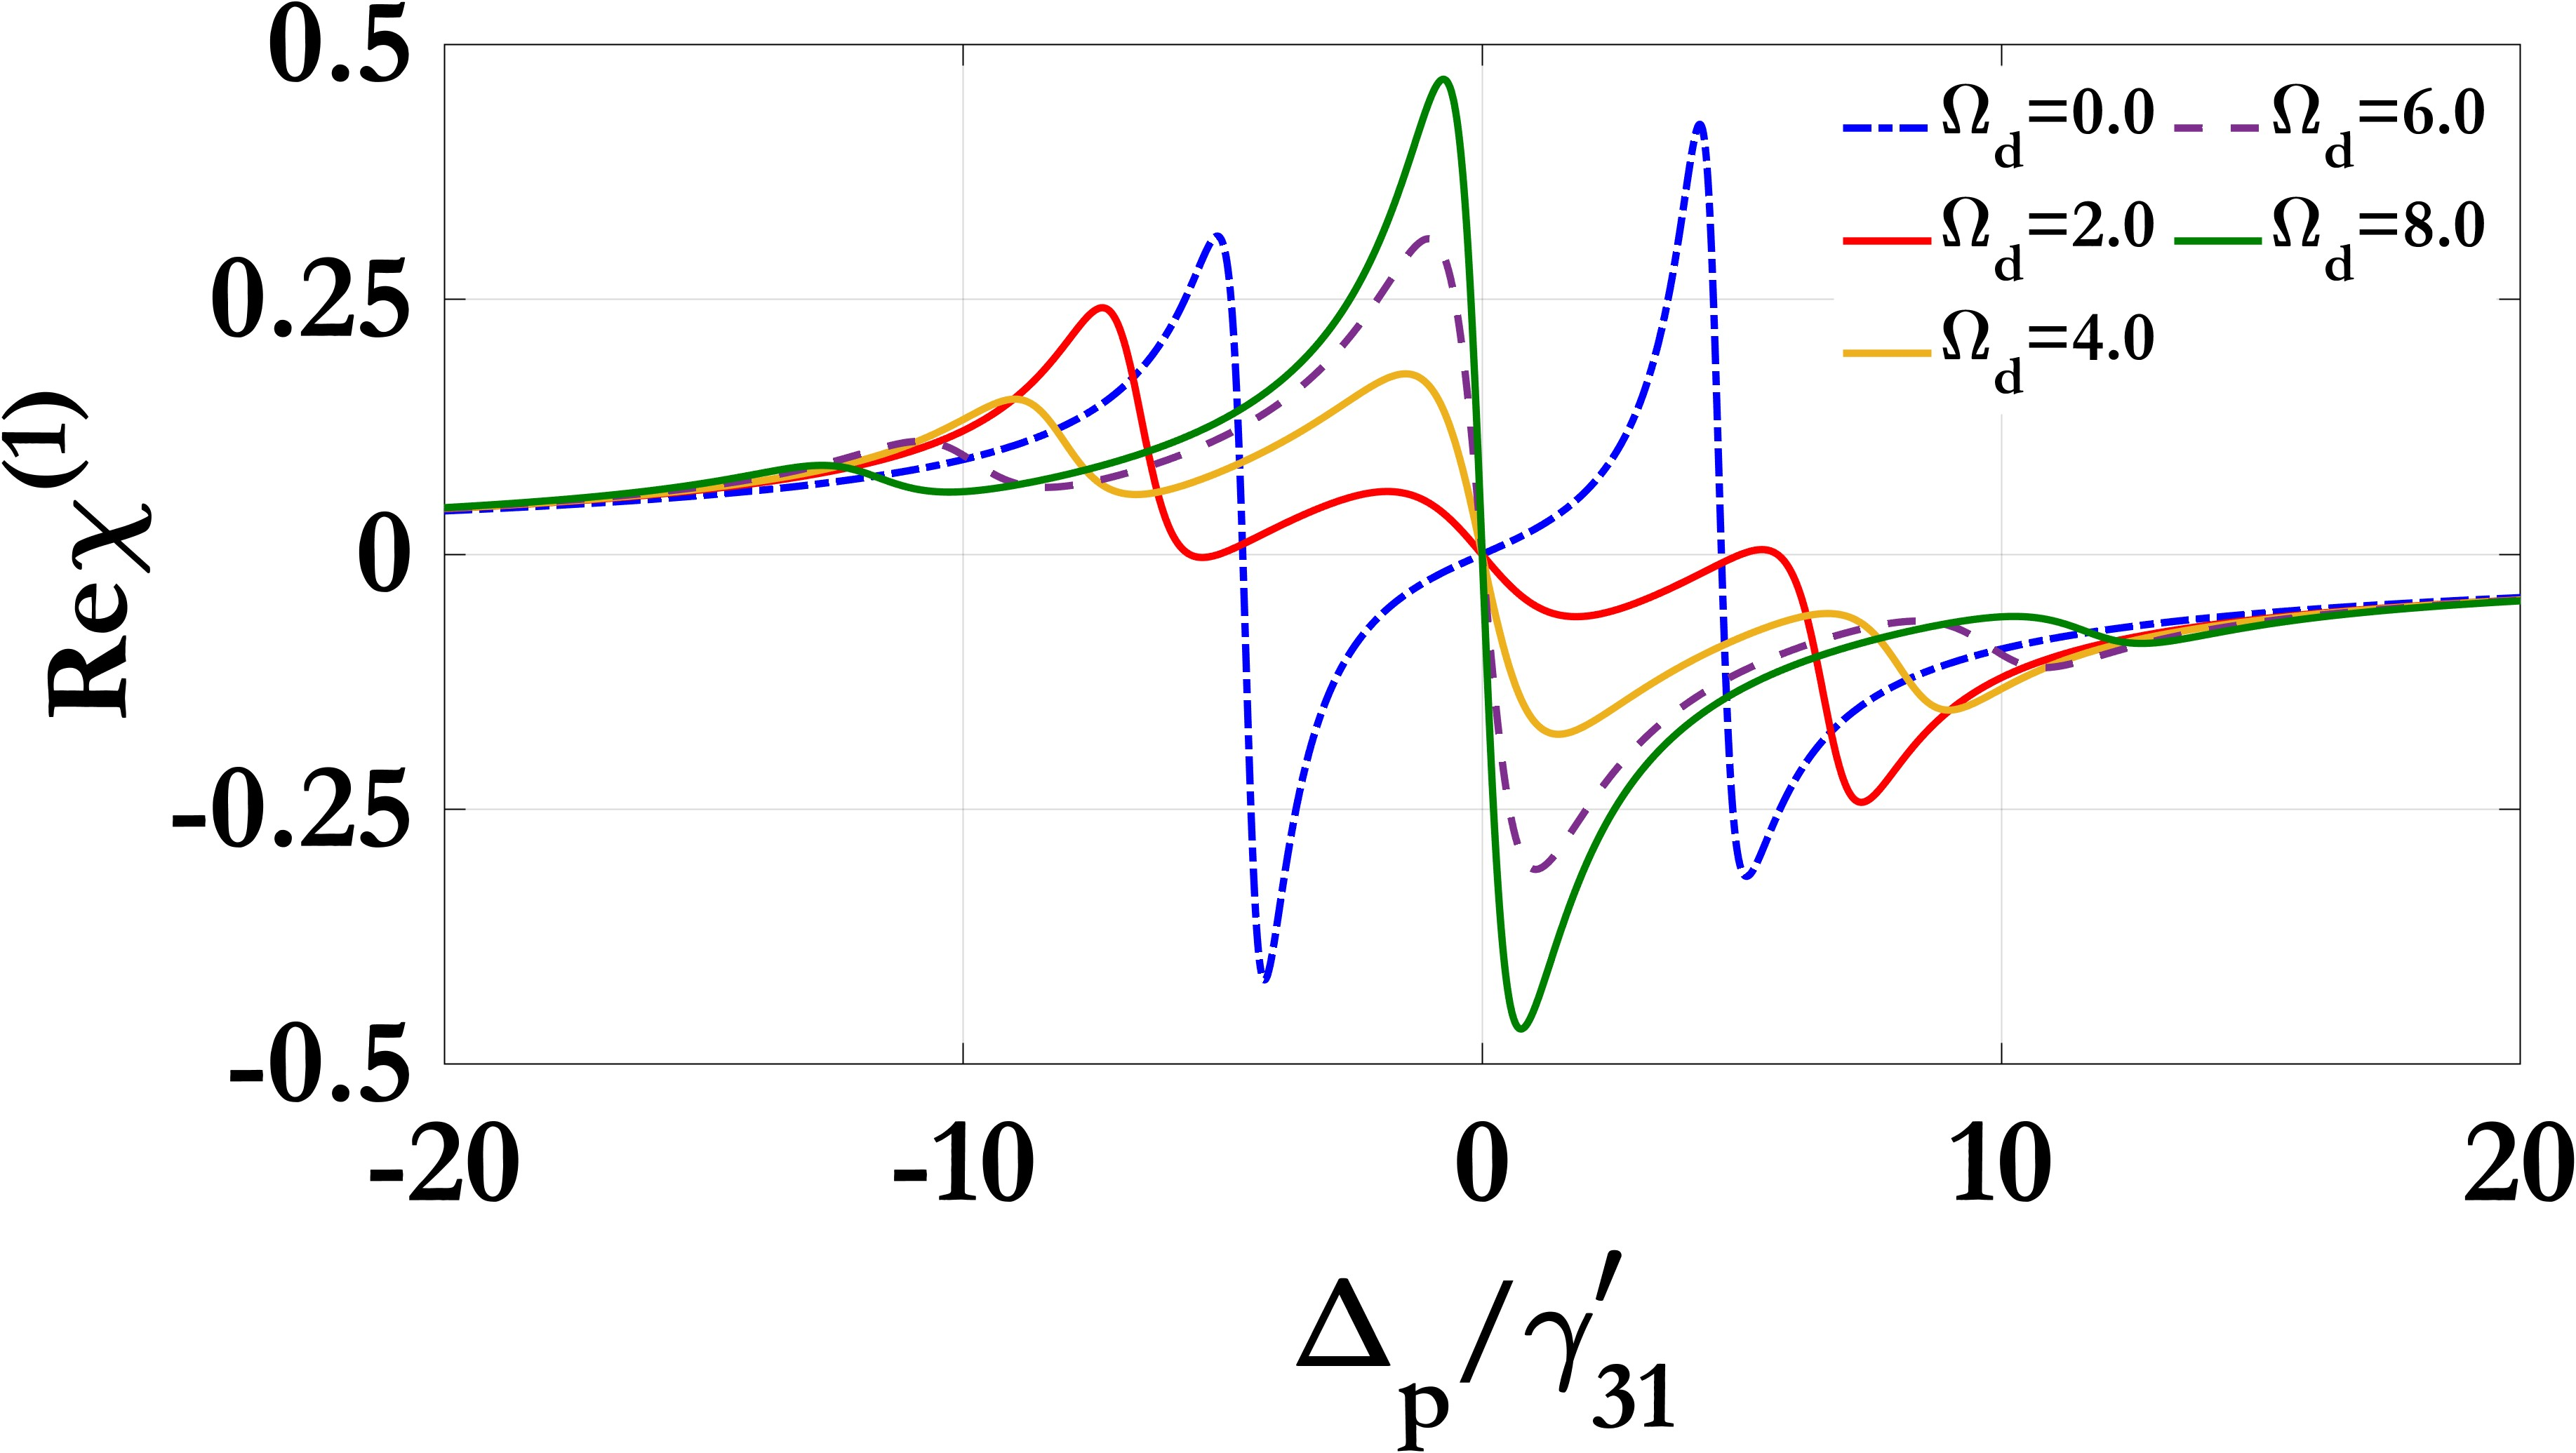
\includegraphics[width=\linewidth]{Plots/Real_chi1_Omega_d.jpeg}
    \subcaption{}
  \end{minipage}
  \caption{Variation of the imaginary (a) and real (b) parts of linear susceptibility as a function of normalized probe detuning for different values of Rabi frequency of second control field ($\Omega_c=0\gamma^{\prime}_{41},\ 1\gamma^{\prime}_{41}$) for imaginary part and ($\Omega_c=2\gamma^{\prime}_{41}$) for real part and Rabi frequency of the third control field is switched off.}
  \label{fig:chi1_omegad}
\end{figure}

In this section we examine the behaviour of linear, Kerr nonliniearities exhibited by multiple SQD-systems at the probe frequency. The value of the several parameters releated to the SQDs are as follows \(\mu_{41} = 15.68\times10^{-29} Cm\), \(\omega_p = 2.84\times10^{14} S^{-1}\). The decay rates are \(\gamma_{21}=3\times10^9S^{-1}\), \( \gamma_{31}=2\times10^9S^{-1} \), \( \gamma_{41}=4.1\times10^{11}S^{-1} \), and the value of the normalization constant is chosen to be \( \gamma^{\prime}_{41}=1\ ps^{-1} \). Before proceeding further we first examine the properties of the linear susceptibilities (\(\chi^{(1)}\)) of the probe beam in absence of relative phase ($\phi$) of the applied fields. In Fig.1(a) we have depicted the variations of the imaginary part of the linear susceptibility with normalized probe detuning ($\Delta_p/\gamma^{\prime}_{41}$) for different values of Rabi frequency of first control field is kept constant at $\Omega_c/\gamma^{\prime}_{41}=0$ and $\Omega_d/\gamma^{\prime}_{41}=1$ and third control field ($\Omega_b$) is switched off. From Fig.1(a), under the resonance (i.e., $\Delta_c = \Delta_b = \Delta_d = 0$), it has shown that in the absence of second control field (i.e., $\Omega_d = 0$) the probe beam experiences large absorption at around $\Omega_p=0$. With the increase in the value of Rabi frequency of second control beam, the width of absorption peak gradually decrease, while side peaks emerges on both sides of the main peak. Consequently, transmission windows are created at the off-resonant positions ($\Delta_p \neq 0$) of the probe beam .The width of these two side windows increases with the increase of the value of $\Omega_d/\gamma^{\prime}_{41}$. Therefore the second control beam is not sufficient to create a transperency window at the probe resonance. Secondary transmission window can be created at off-resonant positions. Fig.1(b) demostrates the variation of the real part of $\chi^{(1)}$ versus normalized probe detuning ($\Delta_p/\gamma^{\prime}_{41}$) for different values of Rabi frequency ($\Omega_{d}$) of second control beam. While Rabi frequency of first and third control field is kept constant at $\Omega_{c}/\gamma^{\prime}_{41}=2$ and $\Omega_{b}/\gamma^{\prime}_{41}=2$ .As shown in Fig.1(b) with the increase in the value of the second control beam $\Omega_{d}$ from $0$ to $8\gamma^{\prime}_{41}$, the slope of the ($Re\chi^{(1)}$) changes and since this slope determines the group velocity of the beam, consequently the group velocity can be controlled by second control beam. \par

\begin{figure}[ht]
  \centering
  \begin{minipage}{0.48\textwidth}
    \centering
    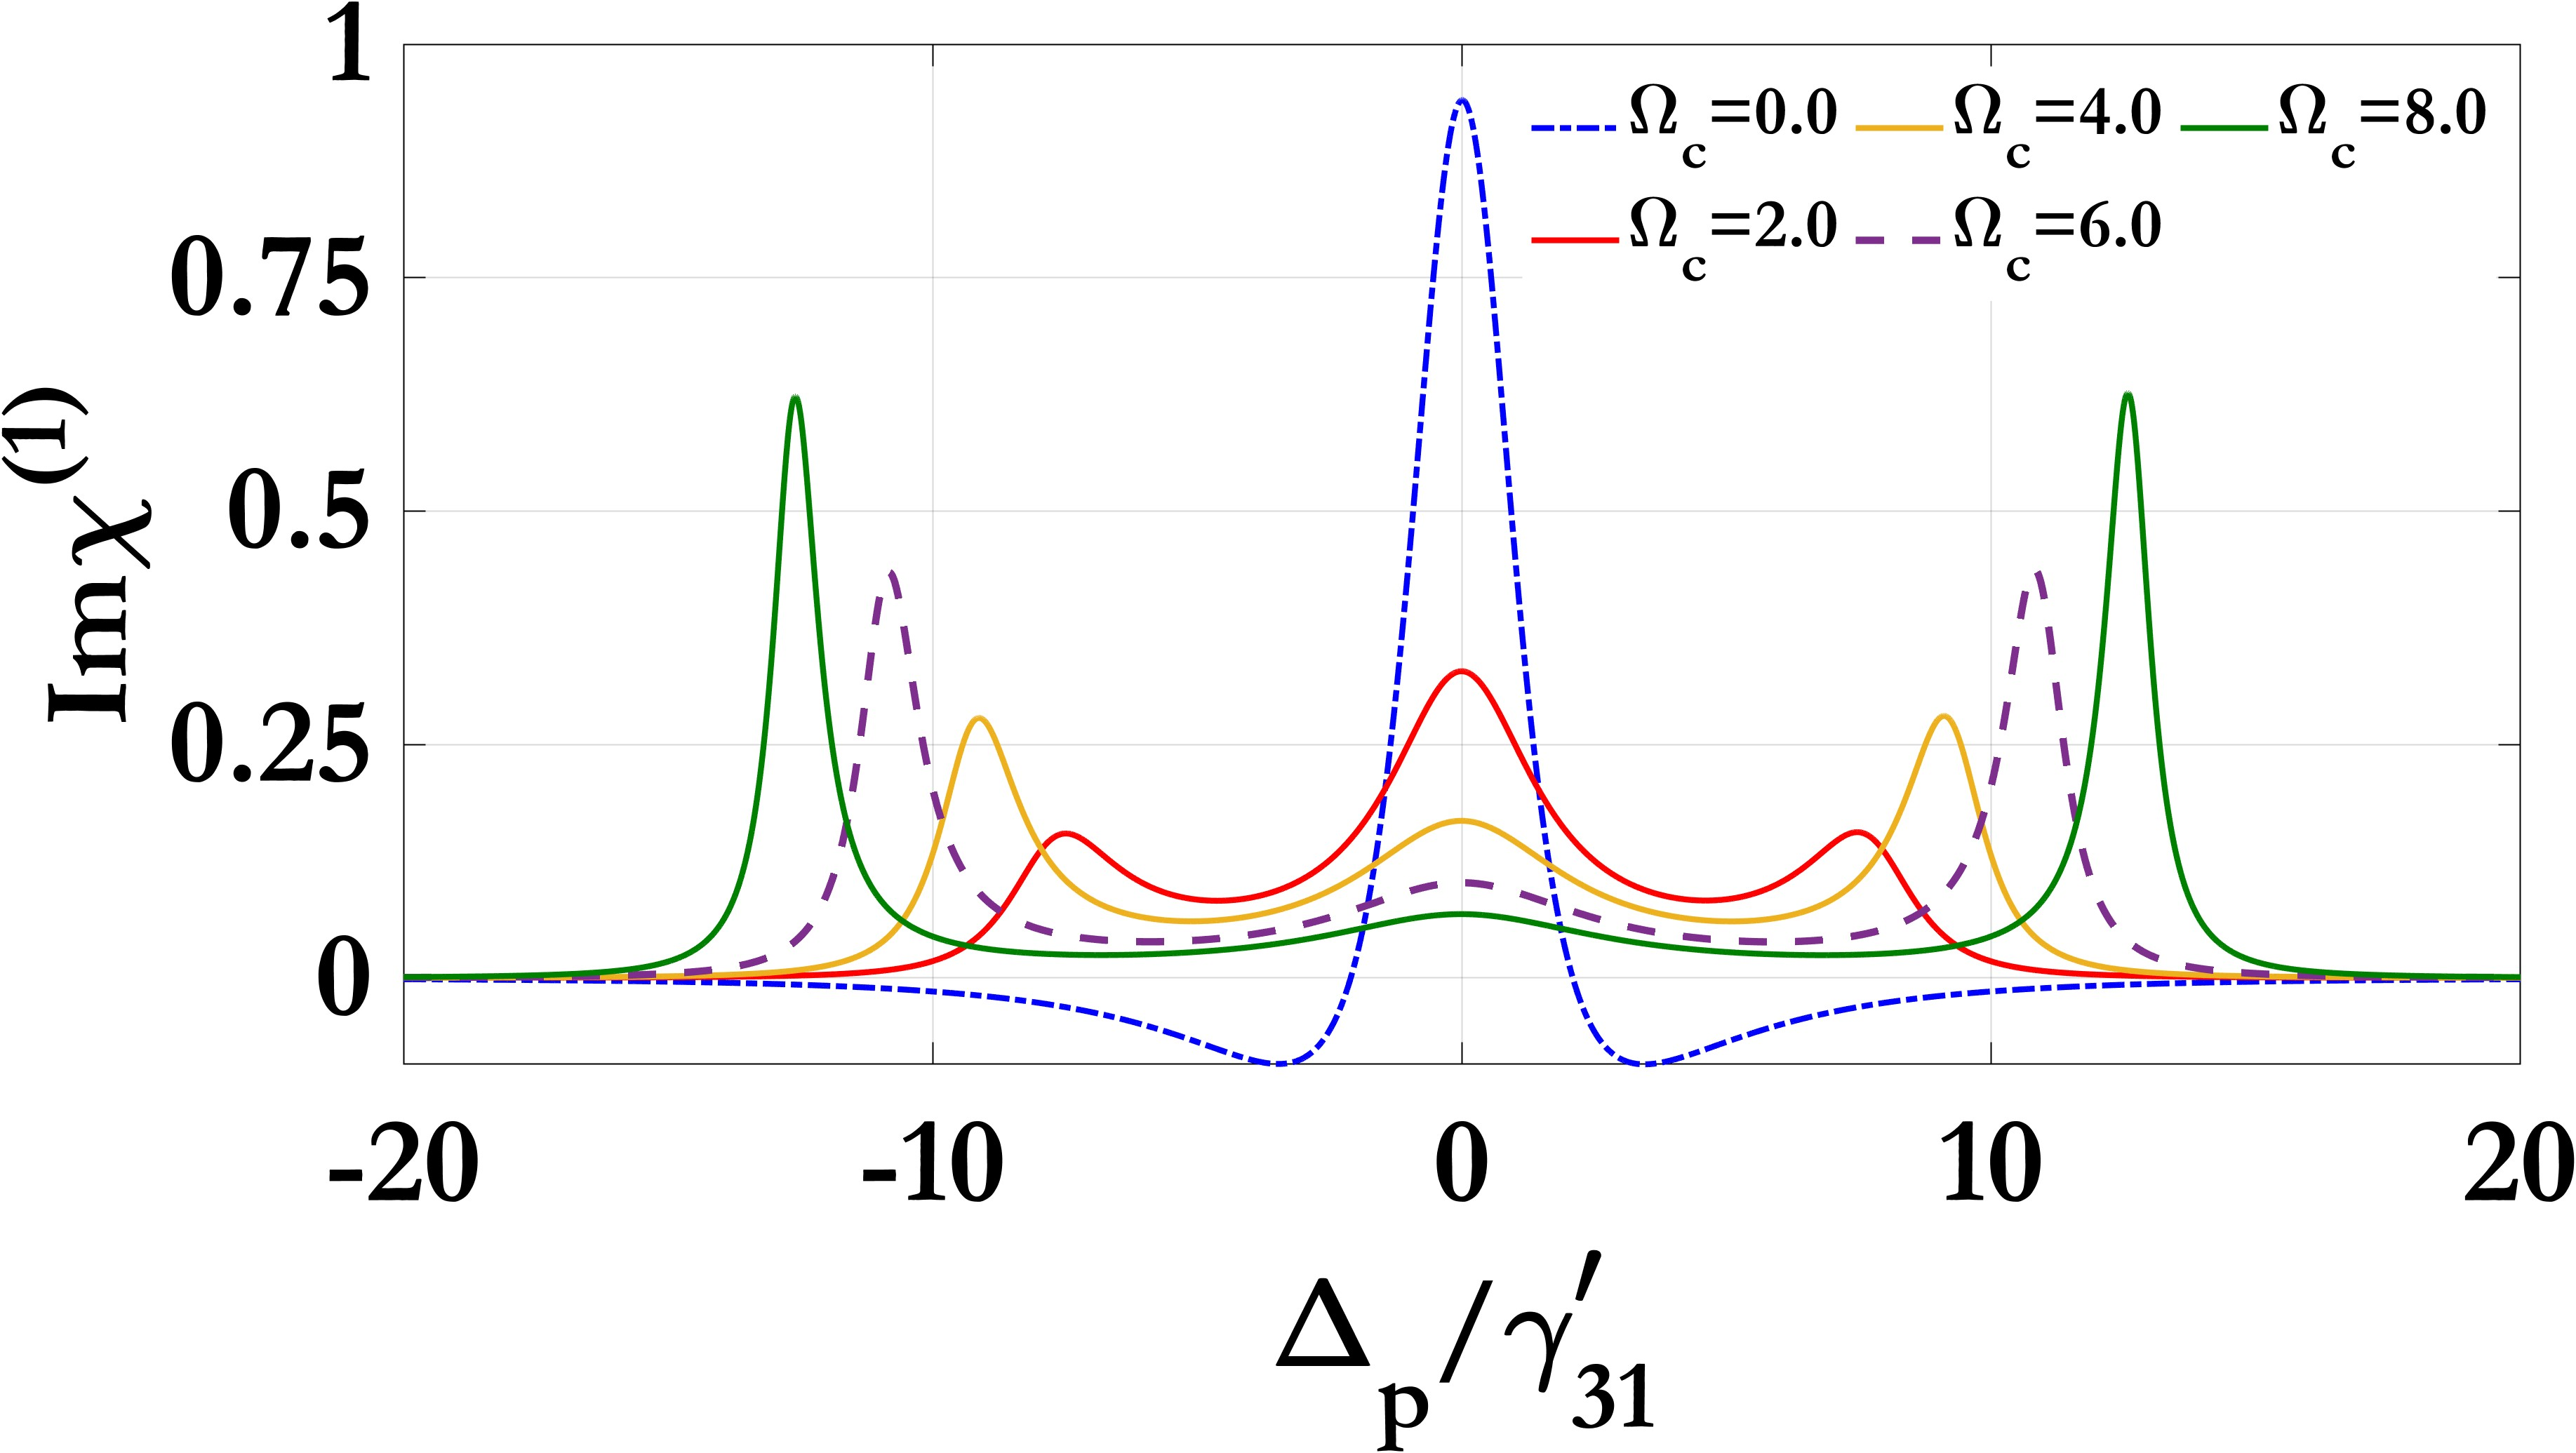
\includegraphics[width=\linewidth]{Plots/Img_chi1_Omega_c.jpeg}
    \subcaption{}
  \end{minipage}%
  \hfill
  \begin{minipage}{0.48\textwidth}
    \centering
    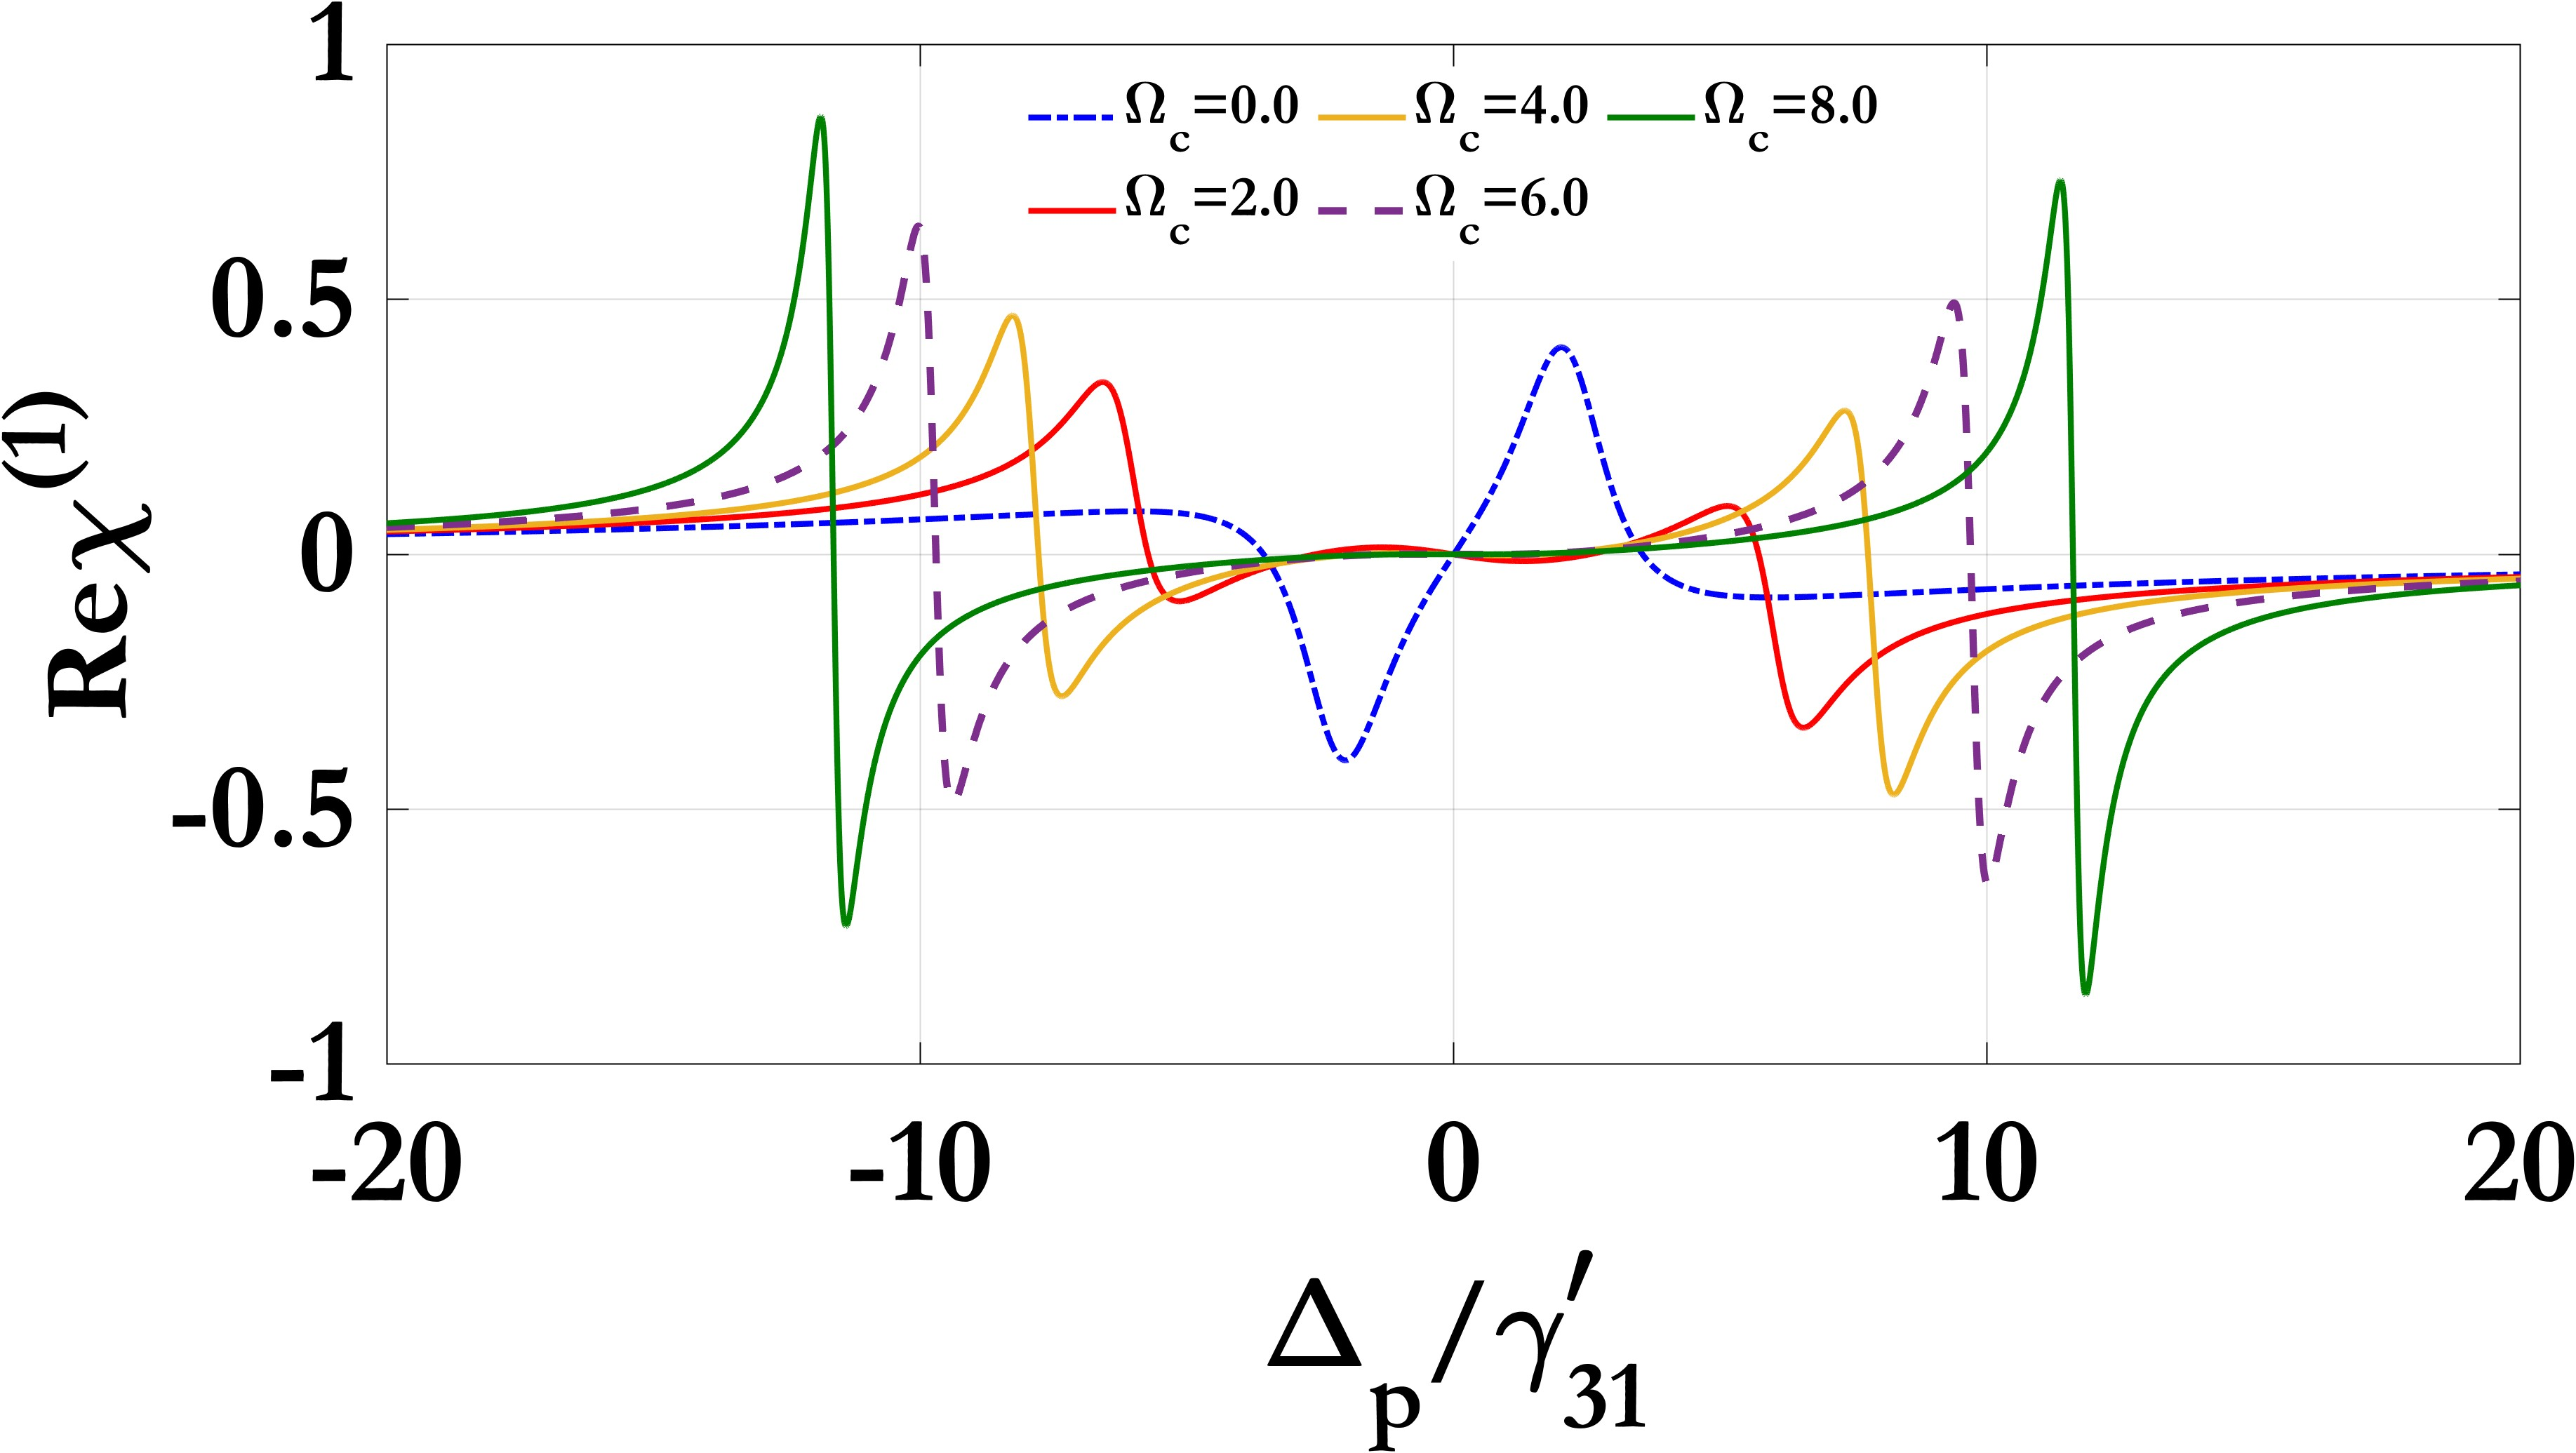
\includegraphics[width=\linewidth]{Plots/Real_chi1_Omega_c.jpeg}
    \subcaption{}
  \end{minipage}
  \caption{Variation of the imaginary (a) and real (b) parts of linear susceptibility as a function of normalized probe detuning for different values of Rabi frequency of second control field ($\Omega_c=0\gamma^{\prime}_{41},\ 1\gamma^{\prime}_{41}$) for imaginary part and ($\Omega_c=2\gamma^{\prime}_{41}$) for real part and Rabi frequency of the third control field is switched off.}
  \label{fig:chi1_omegac}
\end{figure}

We now examine the influence of first control field ($\Omega_{c}$) on the behaviour of linear susceptibility. We have discussed the variations of the imaginary and real part of $\chi^{(1)}$ with normalized probe $\Delta_{p}/\gamma^{\prime}_{41}$ for different values of the Rabi frequency of the first control beam ($\Omega_c$), while the values of other two control field kept constant (i.e. switched off).

From Fig.2(a) we notice that absorption window is created at $\Omega_{c}=0$ when second and third control field are switched off (i.e. $\Omega_{d}=\Omega_{b}=0$). As a result of increasing the value of $\Omega_{c}$ the height of the absorption window is gradually decreasing and also a secondary transparency window is created and the width of the transparency window is increased for higher value of $\Omega_{c}$ and also the height of the transparency window decreases. On the other hand, from Fig.2(b)we find that slope of real $\chi^{(1)}$ changes from negative in the domain $-0.5 \leq \Delta_{p}/\gamma^{\prime}_{41} \leq 0.5$ for $\Omega_{C}/\gamma^{\prime}_{41}=0$ and similar behaviour is observed for the other cases of $\Omega_{c}$.

The influence of the first control field Rabi frequency $\Omega_c$ on the linear susceptibility $\chi^{(1)}$ reveals significant insights into the coherent dynamics of the atomic system. As shown in the real part of the susceptibility, $\mathrm{Re}[\chi^{(1)}]$, an increase in $\Omega_c$ leads to a clear dispersive splitting near the probe detuning $\Delta_p = 0$. At low $\Omega_c$, the dispersion remains broad and relatively featureless, but as $\Omega_c$ is increased, sharp dispersion profiles emerge, with zero crossings shifting symmetrically outward from the origin. This behavior reflects the dressing of atomic levels due to the strong coupling field, where the energy eigenstates of the system split, and their interference leads to pronounced refractive index modulation. Such steep dispersion features are particularly relevant for applications in slow light and enhanced nonlinear optics, where the group velocity and susceptibility gradient play a pivotal role.

In parallel, the imaginary part $\mathrm{Im}[\chi^{(1)}]$, which governs absorption, displays a transition from a single absorption peak at low $\Omega_c$ to a pronounced transparency window as $\Omega_c$ increases. This transparency---centered at $\Delta_p = 0$---emerges from destructive quantum interference between excitation pathways, a hallmark of Electromagnetically Induced Transparency (EIT). As $\Omega_c$ becomes large, the absorption profile evolves into a doublet structure with peaks at detunings proportional to $\Omega_c$. This play of EIT, modulated by the control field strength, offers a tunable platform for manipulating light--matter interactions, thereby enabling dynamic control over absorption and dispersion in multi-level atomic media.

\section{Dispersion Spectra for \(\chi^{(3)}\) }

\begin{figure}[h]
  \centering
  \begin{minipage}{0.48\textwidth}
    \centering
    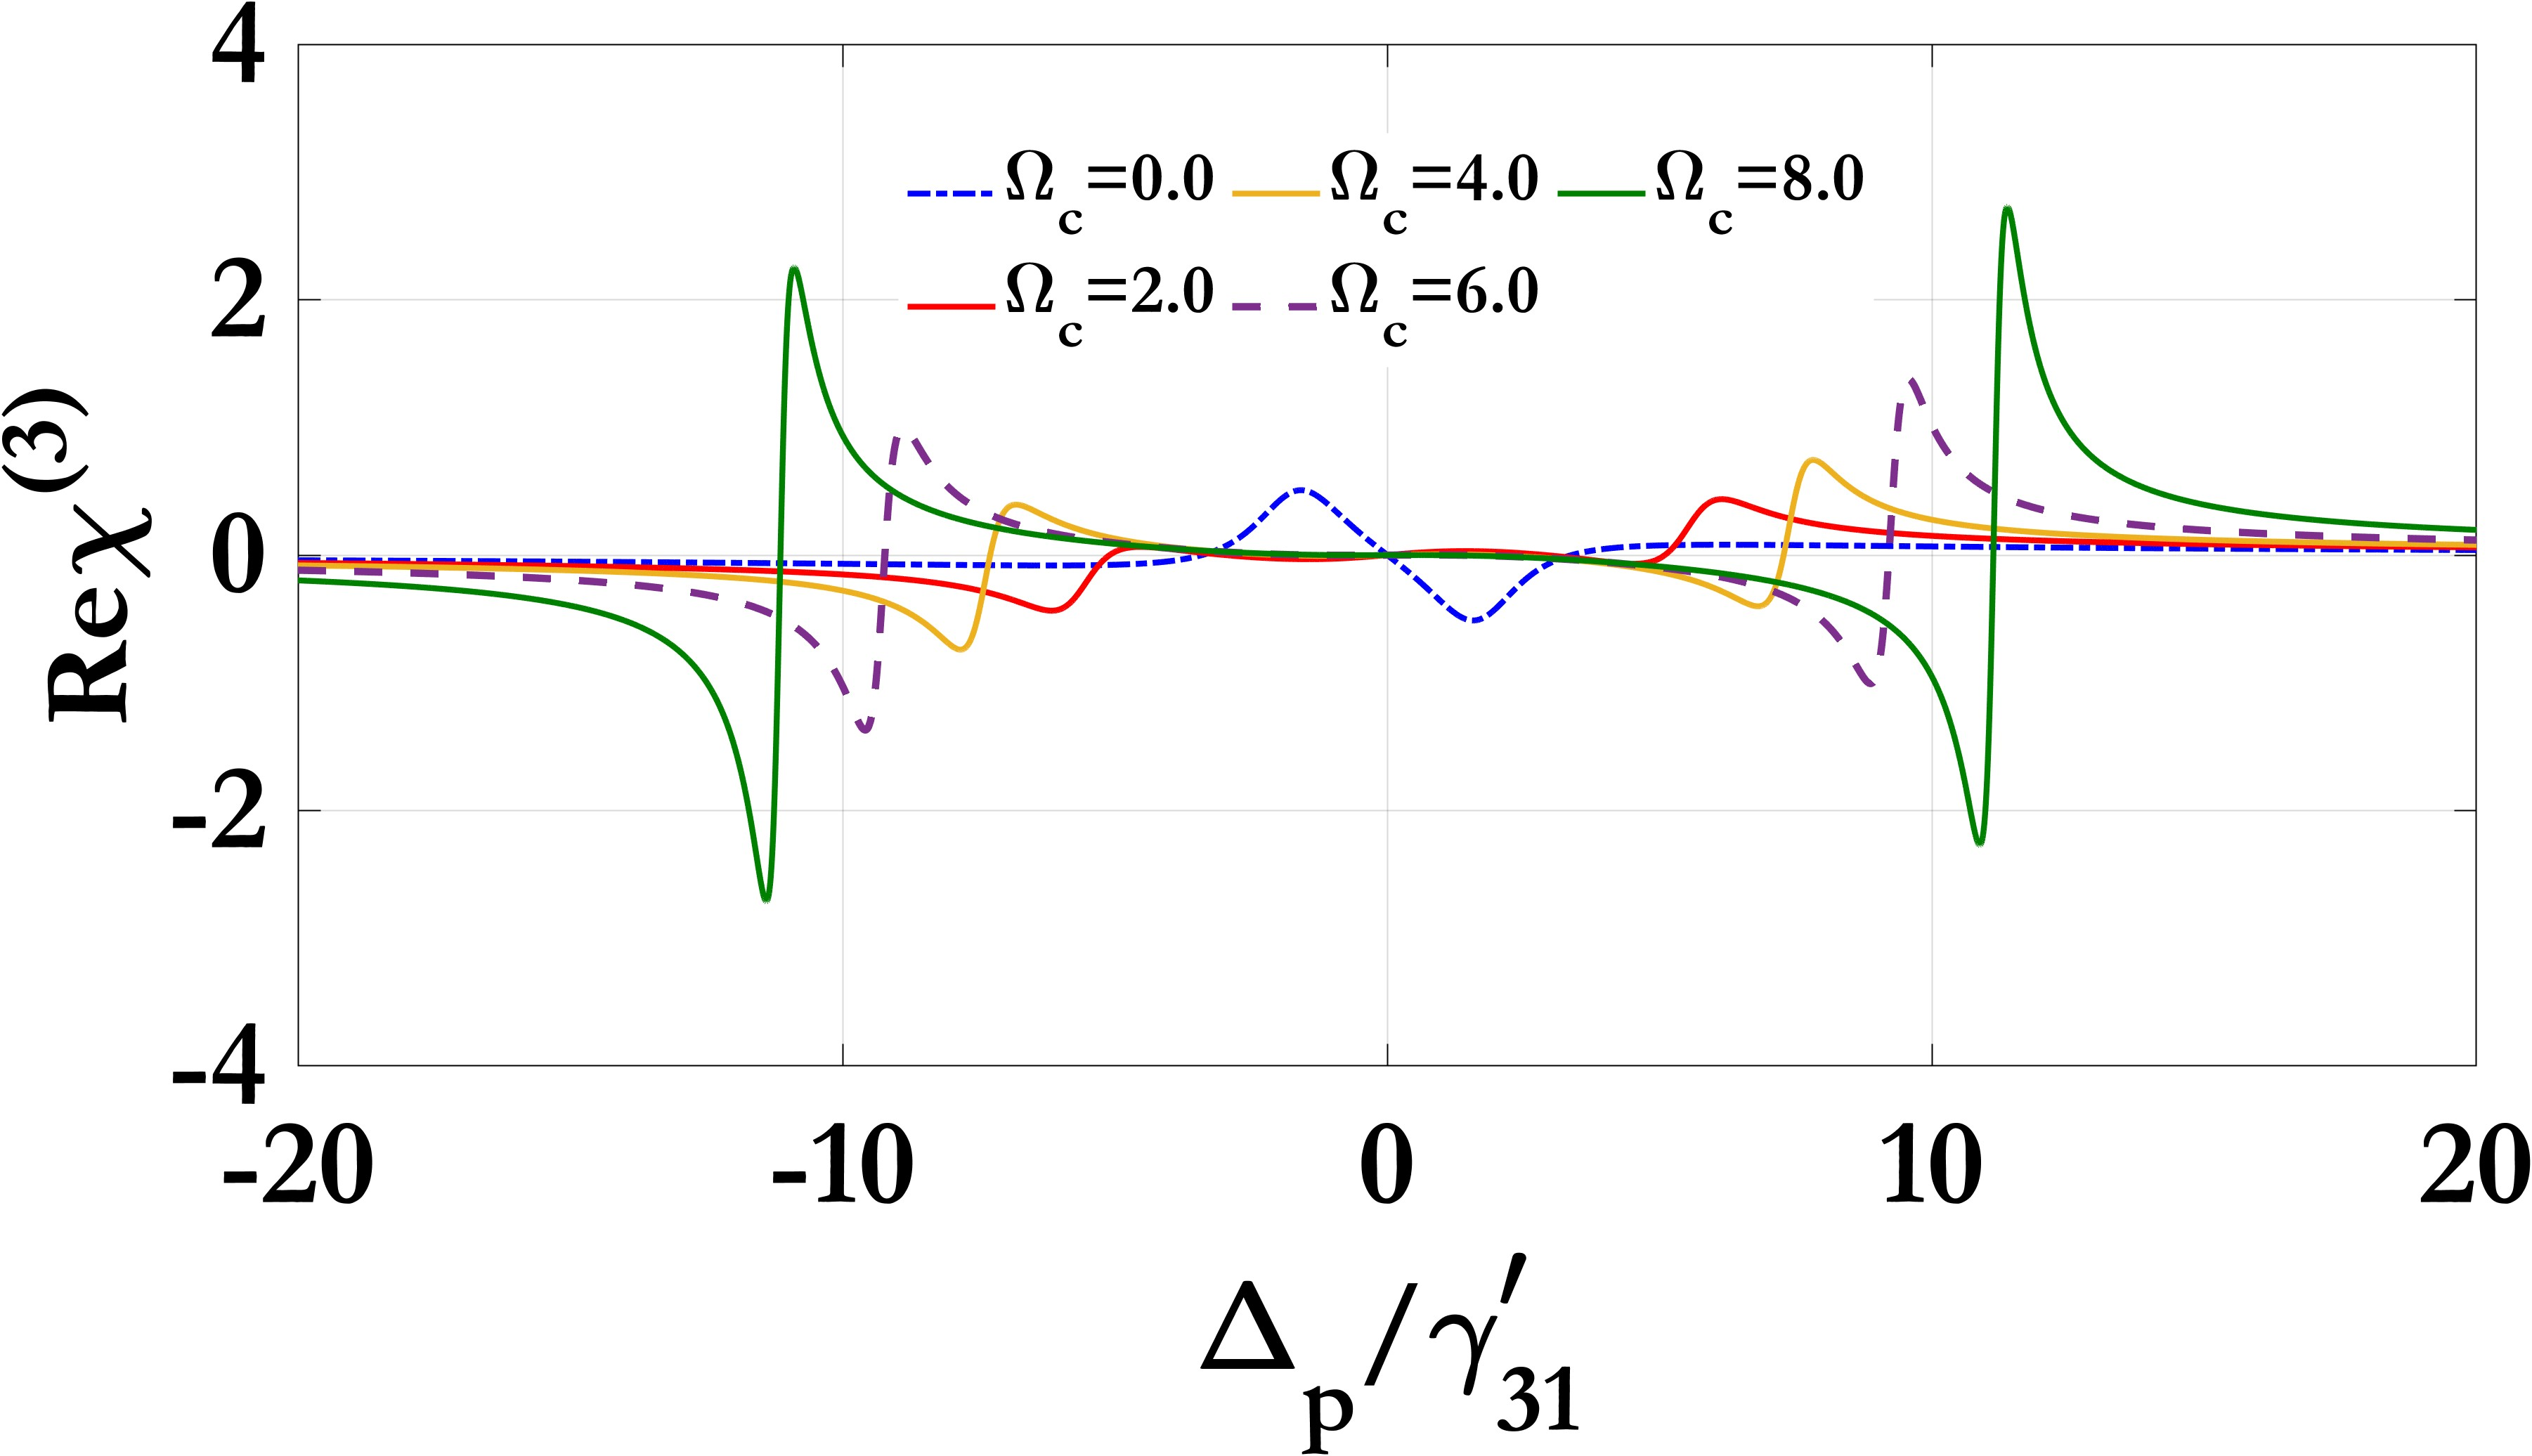
\includegraphics[width=\linewidth]{Plots/Real_chi3_Omega_c.jpeg}
    \subcaption{}
  \end{minipage}%
  \hfill
  \begin{minipage}{0.48\textwidth}
    \centering
    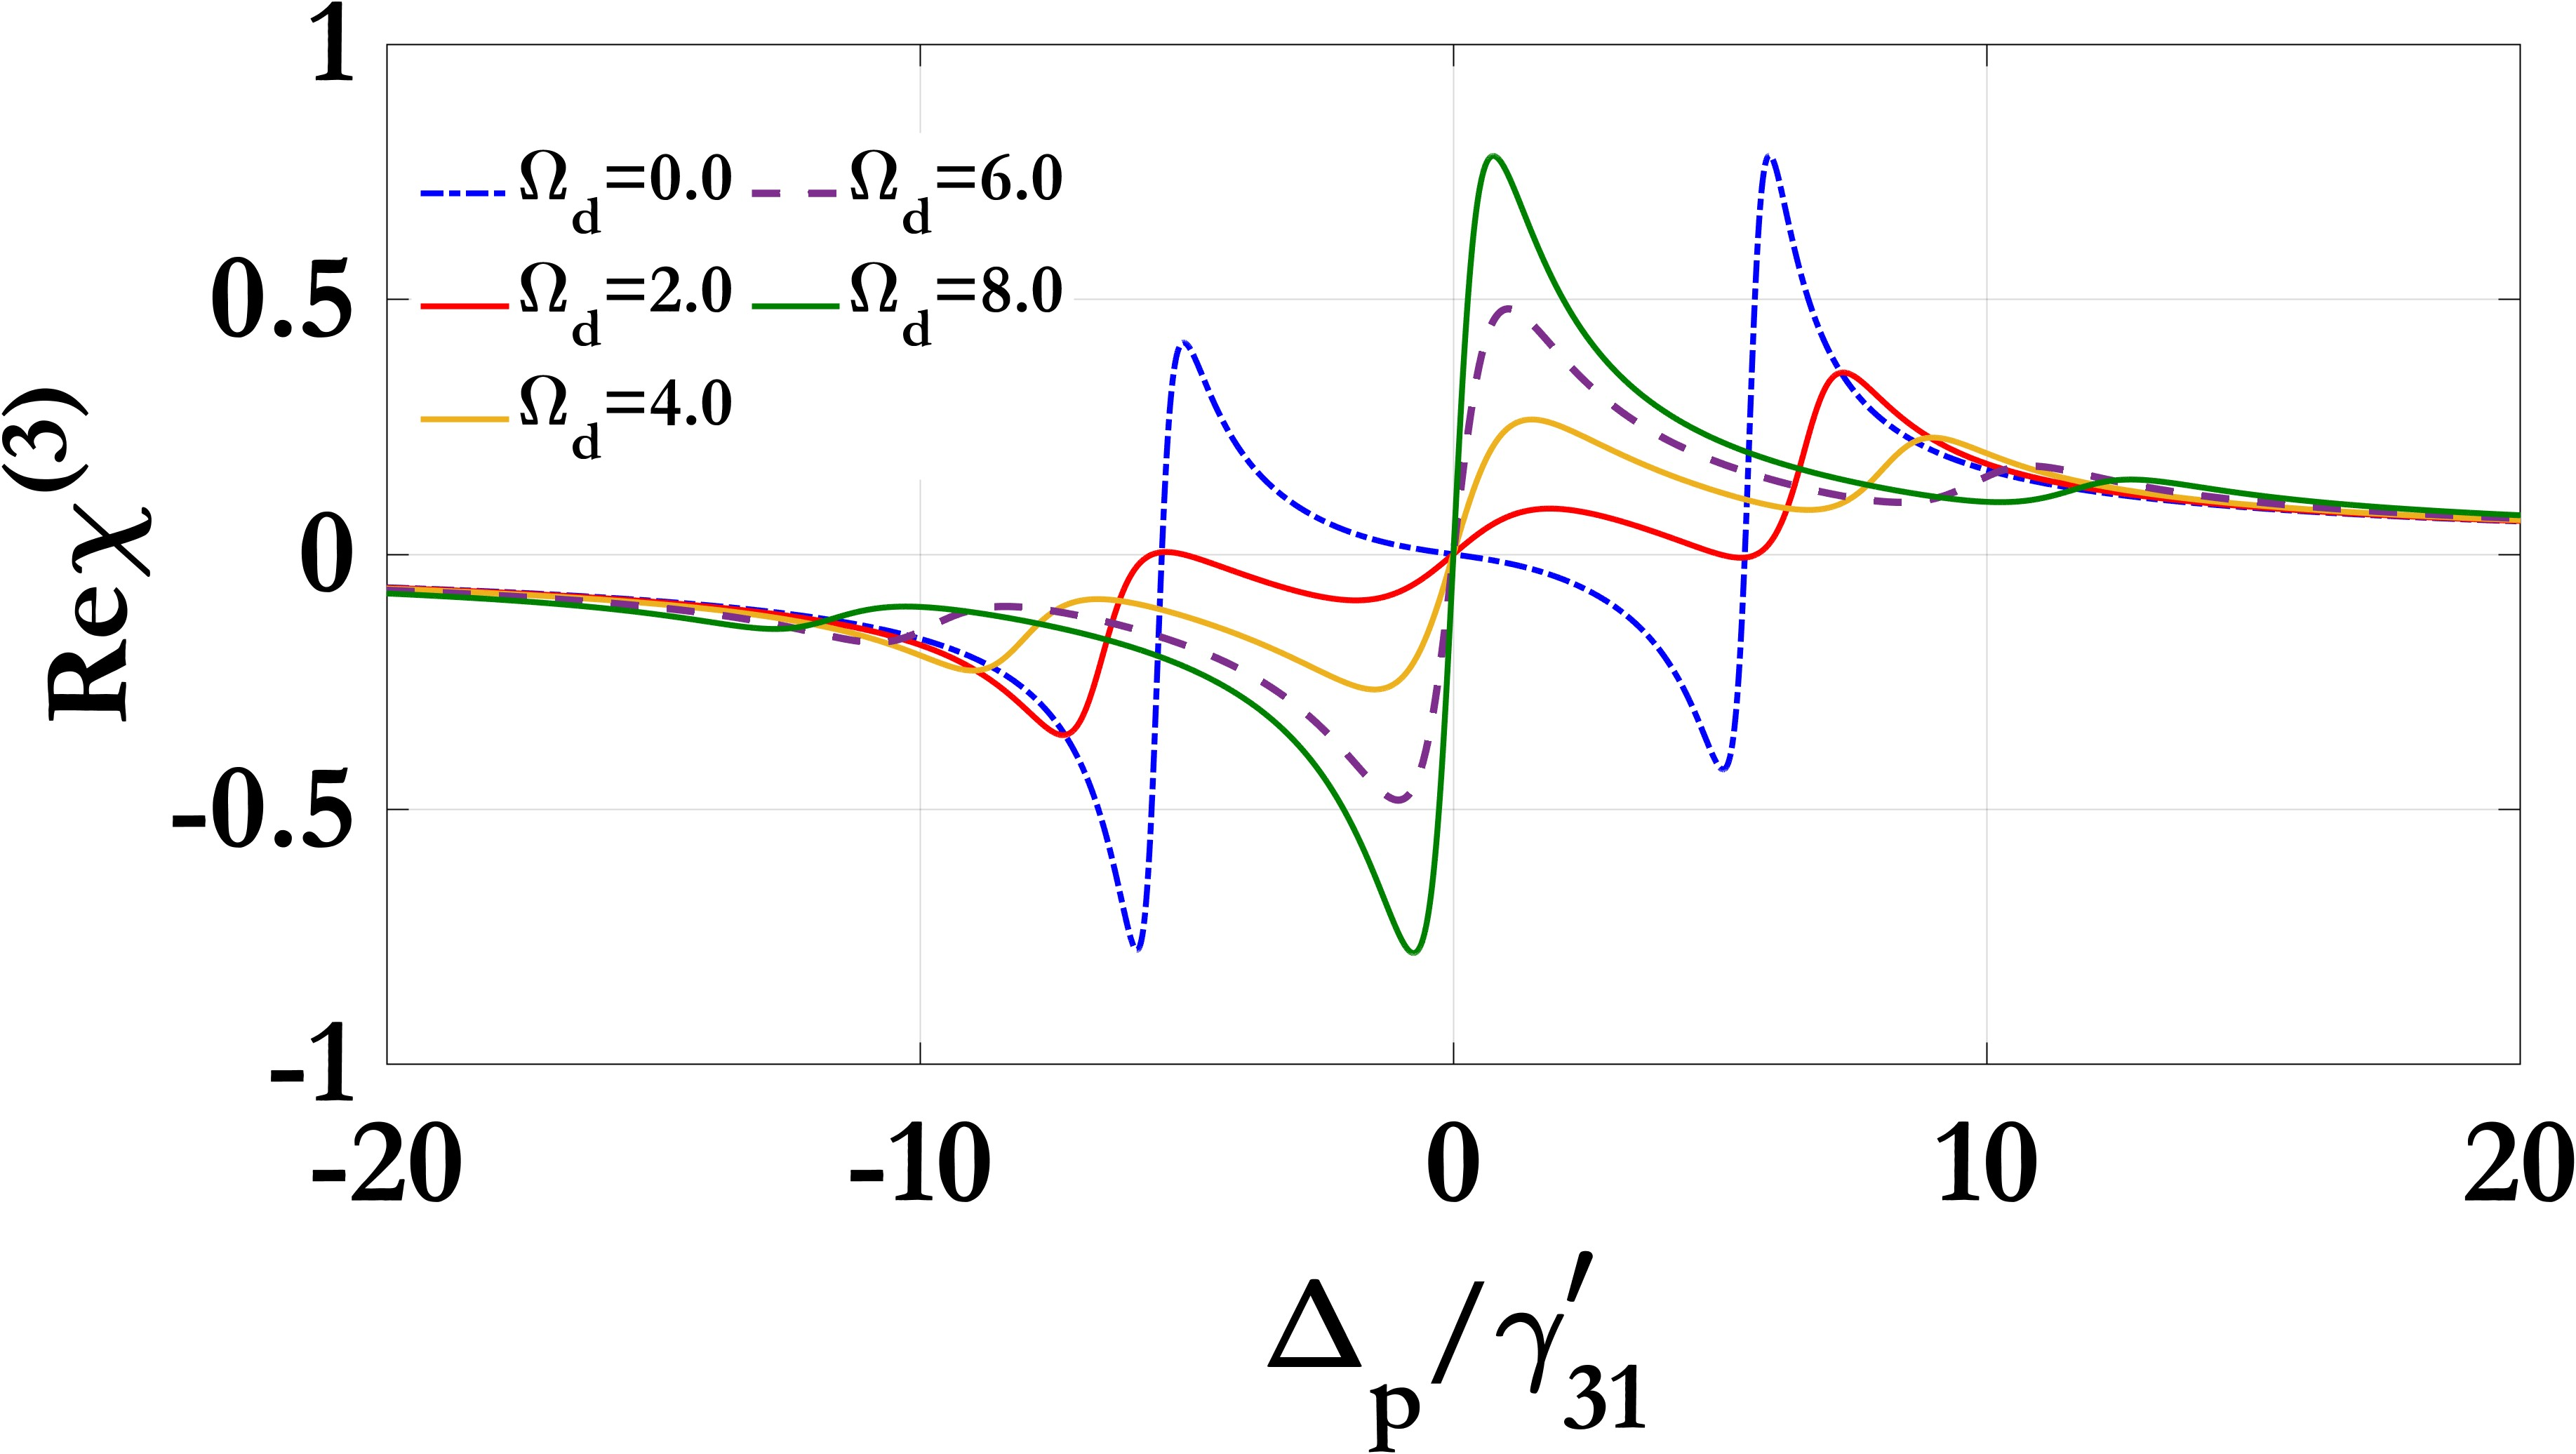
\includegraphics[width=\linewidth]{Plots/Real_chi3_Omega_d.jpeg}
    \subcaption{}
  \end{minipage}
  \caption{Variation of the imaginary (a) and real (b) parts of linear susceptibility as a function of normalized probe detuning for different values of Rabi frequency of second control field ($\Omega_c=0\gamma^{\prime}_{41},\ 1\gamma^{\prime}_{41}$) for imaginary part and ($\Omega_c=2\gamma^{\prime}_{41}$) for real part and Rabi frequency of the third control field is switched off.}
  \label{fig:chi3_omegad}
\end{figure}

The dispersion spectra of the real part of the third-order nonlinear susceptibility, \(\text{Re}\,\chi^{(3)}\), presented in Figs.~X(a) and X(b), provide crucial insight into the underlying nonlinear optical response of the medium under varying Rabi frequencies of the dressing field \(\Omega_d\) and control field \(\Omega_c\), respectively. The system is considered under the fixed detuning conditions \(\Delta_c = 1\), \(\Delta_b = 2\), and \(\Delta_d = 0\), with the normalization factor \(\gamma_{41}^\prime = 1~\text{ps}^{-1}\). These dispersion profiles reveal significant sensitivity of the real part of \(\chi^{(3)}\) to the external driving fields, reflecting the tunable nature of the Kerr-type nonlinearity via coherent field control. As \(\Omega_d\) and \(\Omega_c\) are varied, one observes pronounced dispersive features—including polarity flips and sharp peaks—indicative of enhanced multi-photon coherence and interference effects among dressed atomic states. These features correspond to rapid variations in the refractive index and group velocity dispersion, which are foundational for phase-sensitive nonlinear phenomena such as four-wave mixing and cross-phase modulation.

More specifically, increasing \(\Omega_d\) or \(\Omega_c\) results in enhanced splitting and asymmetry in the dispersion profiles, a manifestation of strong Autler--Townes splitting and dynamic Stark shifts in the atomic energy levels. The observed spectral modulations point to the presence of both normal and anomalous dispersion regions, corresponding respectively to subluminal and superluminal group velocity regimes. Importantly, the field-dependent tailoring of \(\text{Re}\,\chi^{(3)}\) opens avenues for precise engineering of nonlinear optical responses, crucial for developing applications such as all-optical switching, tunable delay lines, and quantum phase gates. The ability to dynamically control the third-order susceptibility without introducing significant absorption further emphasizes the practicality of this scheme in low-power, high-coherence quantum photonic systems.

\section{Modulation instability of Probe Field}

In this section we now proceed to investigate the modulation instability of the CW or QCW probe field. The steady state solution of Eqn. (40) can be written as,
\begin{equation}
A(\xi, T) = \sqrt{P_0} e^{i (\gamma P_0 + \delta P_0^2) \xi}
\tag{41}
\end{equation}
To examine whether the continuous wave (CW) probe beam is stable under small perturbation, we introduce a small perturbation in the following form:
\begin{equation}
A(\xi, T) = \left\{ \sqrt{P_0} + a(\xi, T) \right\} e^{i (\gamma P_0 + \delta P_0^2) \xi}
\tag{42}
\end{equation}
Here \( \sqrt{P_0} \) and \( a(\xi, T) \) are respectively the amplitudes of the CW probe beam in the steady state and small perturbation. The substitution of Eq. (42) in Eq. (40) and subsequent linearization leads to the following equation for the perturbation \( a(\xi, T) \):
\begin{equation}
i \frac{\partial a}{\partial \xi} - \frac{\beta_2(0)}{2!} \frac{\partial^2 a}{\partial T^2} - \frac{i}{3!} \beta_3(0) \frac{\partial^3 a}{\partial T^3} + \frac{1}{4!} \beta_4(0) \frac{\partial^4 a}{\partial T^4} + (\gamma P_0 + 2 \delta P_0^2)(a + a^*) = 0
\tag{43}
\end{equation}
We assume the following solution of the perturbation \( a(\xi, T) \)
\begin{equation}
a(\xi, T) = C e^{i(K \xi - \Omega T)} + D e^{-i(K \xi - \Omega T)}
\tag{44}
\end{equation}
where \( C \) and \( D \) are the amplitudes of the small perturbation. \( K \) and \( \Omega \) are wave number and frequency of the perturbation. By virtue of Eqs. (43) and (44), we get the following two homogeneous equations for \( C \) and \( D \):
\begin{equation}
C(-K + G) + (\gamma P_0 + 2 \delta P_0^2) D = 0
\tag{45}
\end{equation}
\begin{equation}
(\gamma P_0 + 2 \delta P_0^2) C + (K + \tilde{G}) D = 0
\tag{46}
\end{equation}
where,
\[
G = \left[ \frac{\beta_2(0)}{2!} \Omega^2 + \frac{\beta_3(0)}{3!} \Omega^3 + \frac{\beta_4(0)}{4!} \Omega^4 + (\gamma P_0 + \delta P_0^2) \right]
\]
\[
\tilde{G} = \left[ \frac{\beta_2(0)}{2!} \Omega^2 - \frac{\beta_3(0)}{3!} \Omega^3 + \frac{\beta_4(0)}{4!} \Omega^4 + (\gamma P_0 + \delta P_0^2) \right]
\]
The nontrivial solution of Eqs. (45) and (46) for the wave number leads to the dispersion relation:
\begin{equation}
K = \frac{1}{2} \beta_3(0) \Omega^3 \pm i \left\{ \left[ \left( \frac{\beta_2(0)}{2!} \Omega^2 + \beta_4(0) \frac{\Omega^4}{4!} \right) \left( \gamma P_0 + 2 \delta P_0^2 \right) \right] - \left( \frac{\beta_2(0)}{2!} \Omega^2 \right)^2 \right\}^{1/2}
\tag{47}
\end{equation}
The gain of the modulation instability (MI) at frequency \( \Omega \) is given by,

\begin{equation}
g(\Omega) = 2 \times \text{Im}(K)
\tag{48}
\end{equation}
\begin{equation}
g = 2 \left[ \left\{ \beta_2(0) \Omega^2 + \beta_4(0) \frac{\Omega^4}{4!} \right\} \left\{ \gamma P_0 + 2 \delta P_0^2 \right\} - \left\{ \beta_2(0) \frac{\Omega^2}{2!} + \beta_4(0) \frac{\Omega^4}{4!} \right\} \right]^{1/2}
\tag{49}
\end{equation}
The instability gain maximizes at $\Omega_m$ is given by,
\begin{equation}
\Omega_m = \left[ 6 \left\{ \left( \frac{\beta_2}{\beta_4} \right)^2 + \frac{2}{3} \text{frac} \left( (\gamma + 2\delta P_0) P_0 \beta_4 \right) \right\}^{1/2} - 6 \frac{\beta_2}{\beta_4} \right]^{1/2}
\tag{50}
\end{equation}

\begin{figure}[h]
  \centering
  \begin{minipage}{0.48\textwidth}
    \centering
    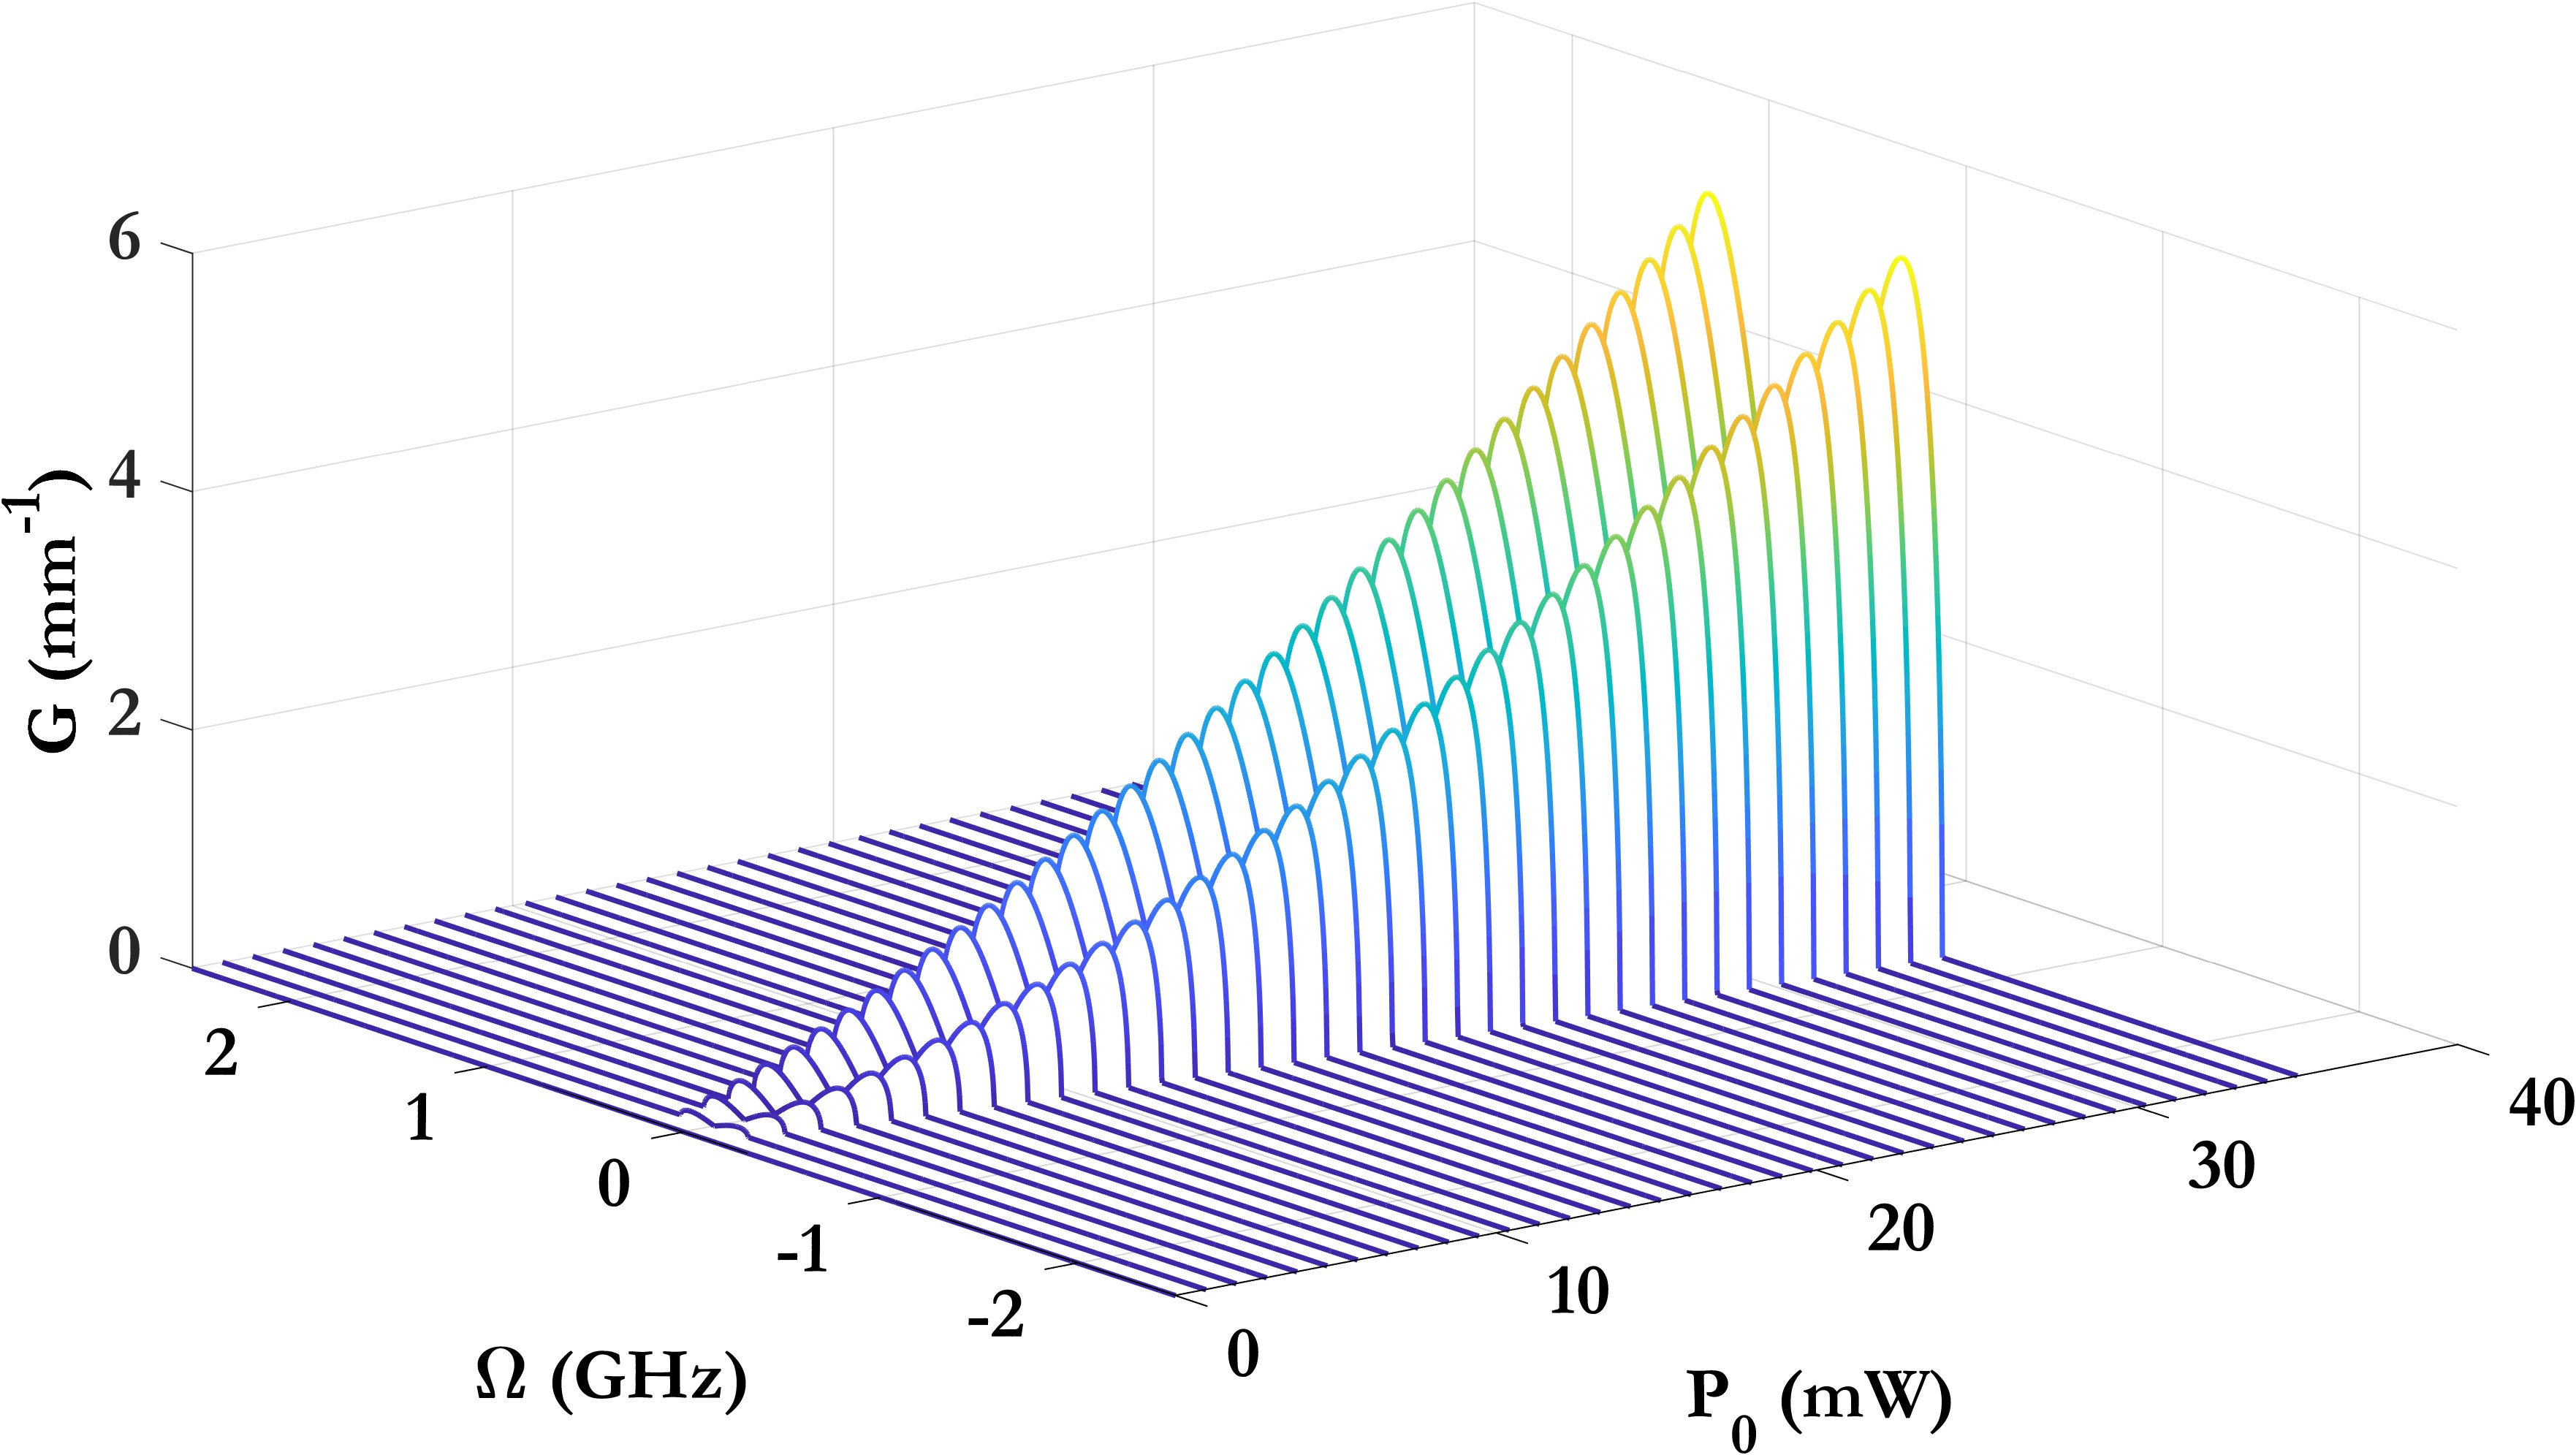
\includegraphics[width=\linewidth]{Plots/Beta2_Kerr.jpeg}
    \subcaption{}
  \end{minipage}%
  \hfill
  \begin{minipage}{0.48\textwidth}
    \centering
    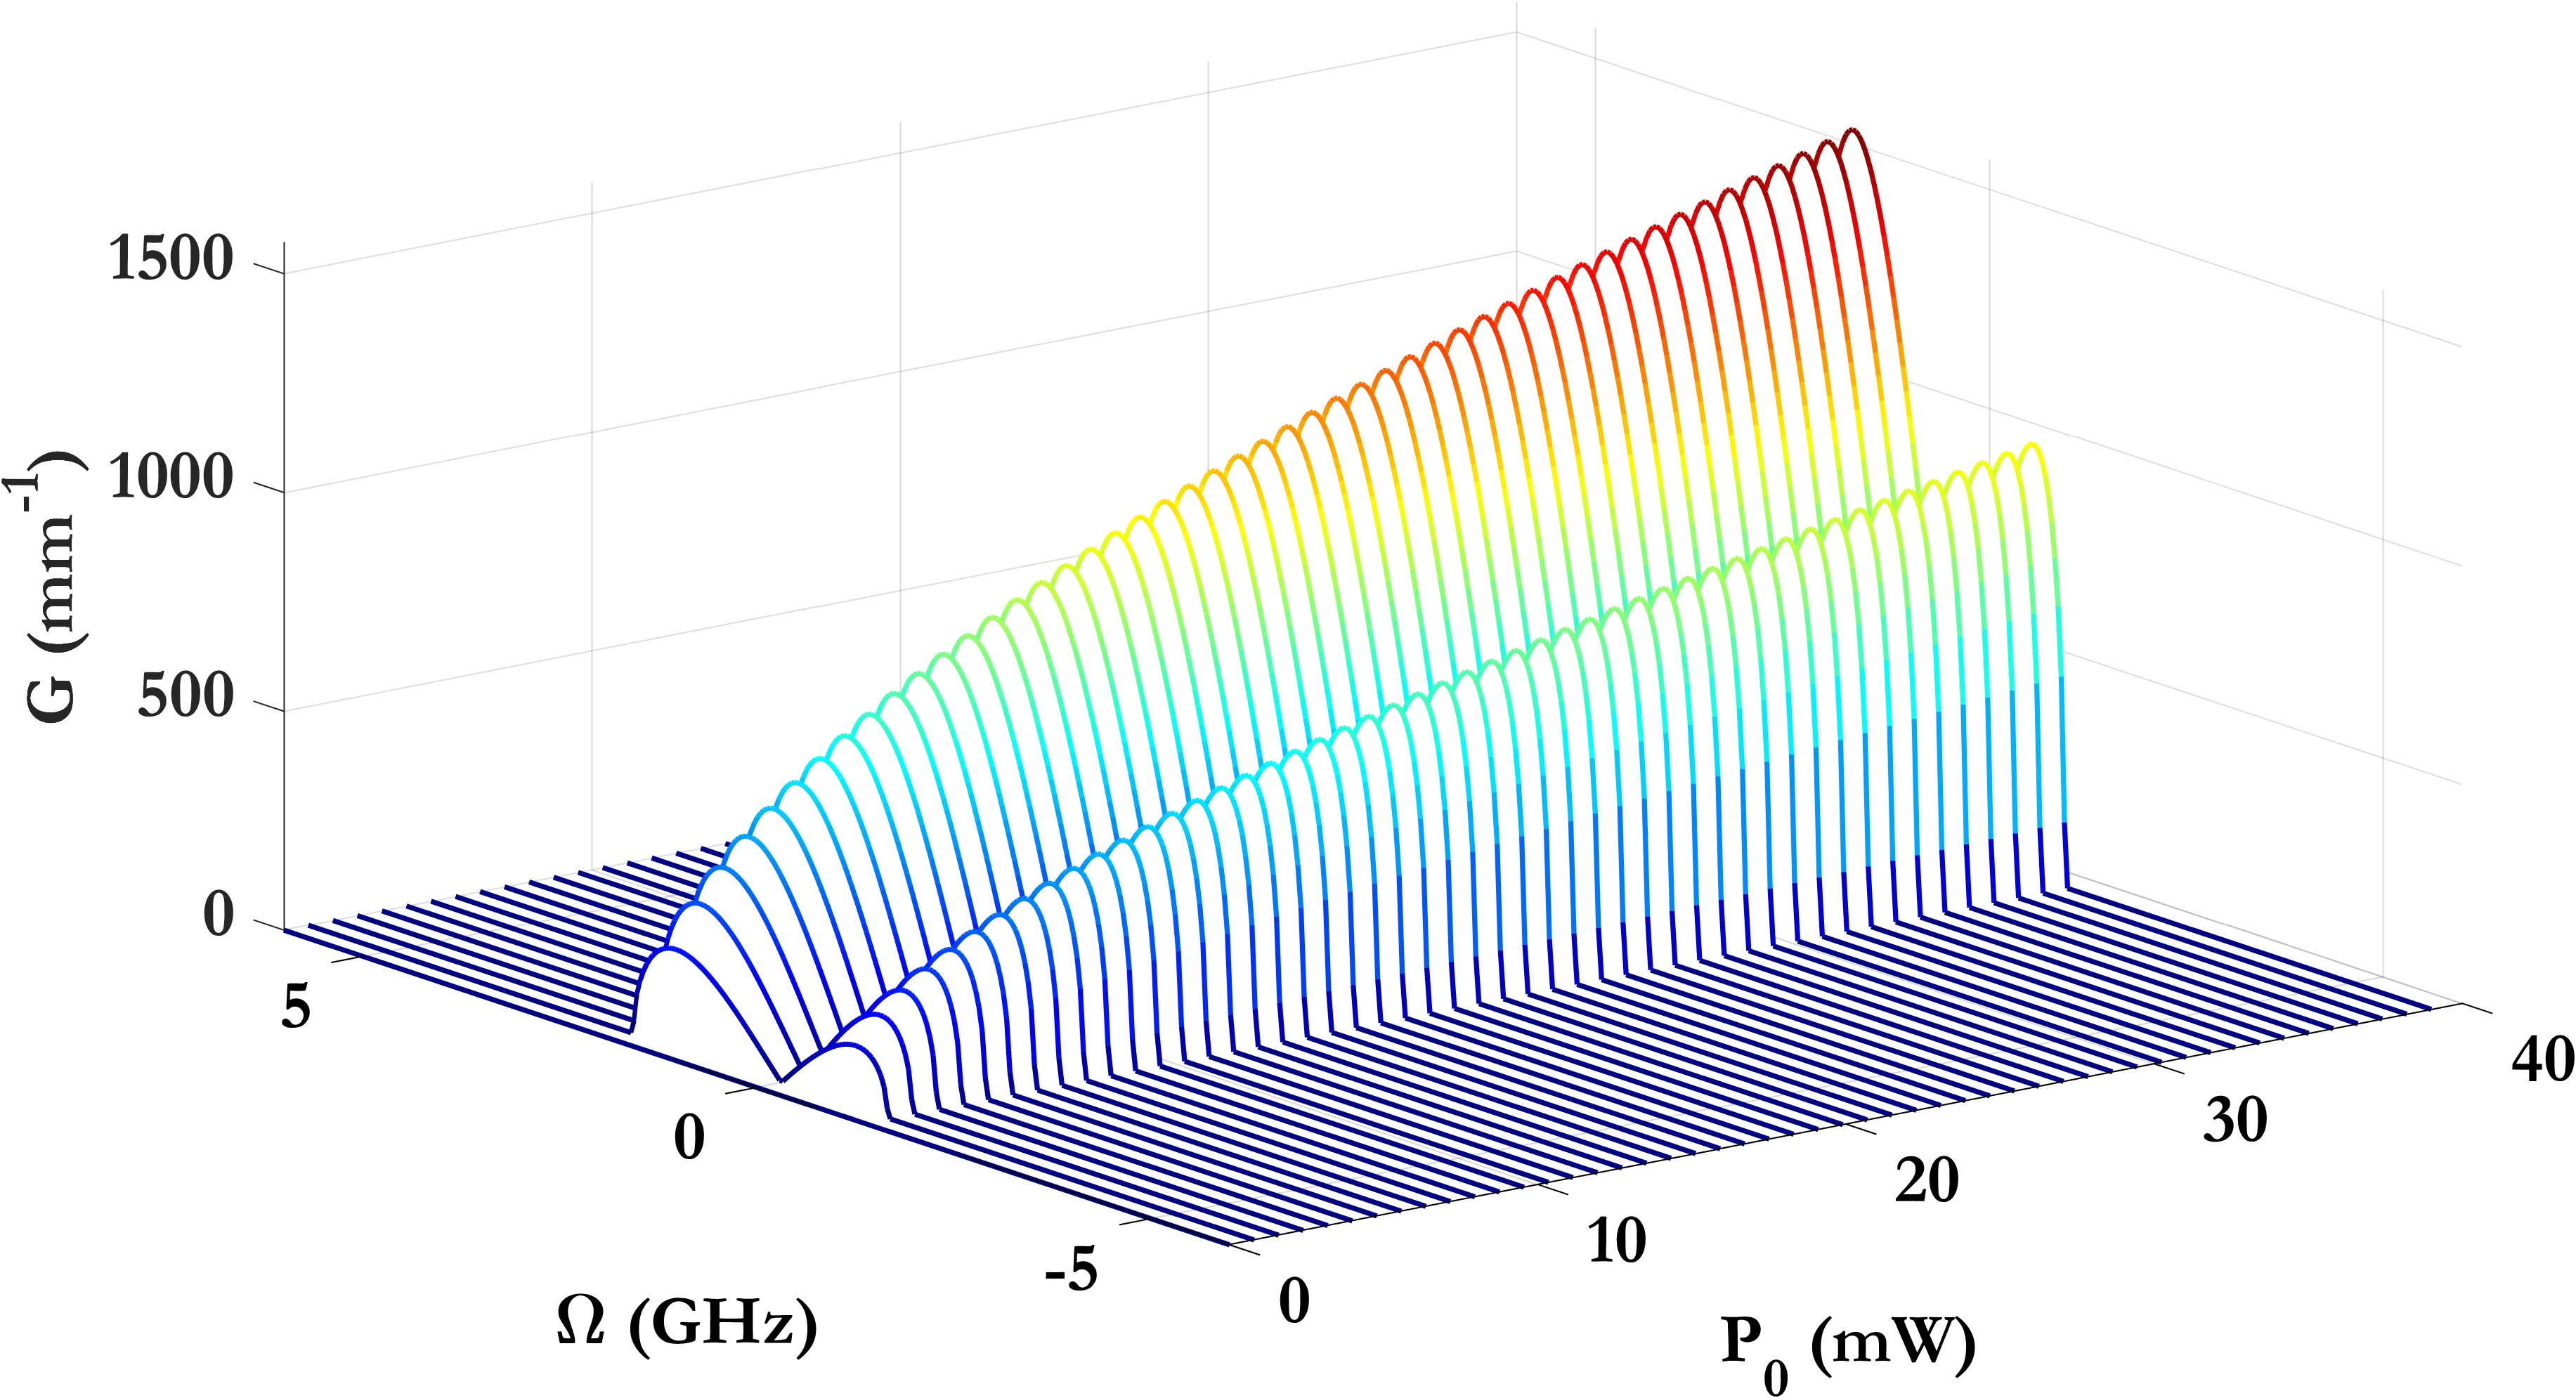
\includegraphics[width=\linewidth]{Plots/Beta4_Kerr.jpeg}
    \subcaption{}
  \end{minipage}
  \caption{Variation of MI gain with the frequency and power in absence and presence of fourth order dispersion (i.e., \(\beta_4=0\) ). (a) In absence of \(\beta_4\), only Kerr nonlinearity present and both Kerr and quintic nonlinearities are present. (b) In presence of \(\beta_4\), only Kerr nonlinearity present and both Kerr and quintic nonlinearities are present.}
  \label{fig:gain}
\end{figure}

\section{Gain Variation w.r.t Frequency for Kerr}



\end{document}
